\section{Notificaciones}

\subsection{Envío de notificaciones}

Cuando la \acrshort{api} procesa alguna de las acciones listadas en el \cref{req:notificaciones} genera una notificación. En la creación de esta notificación la \acrshort{api} busca en la base de datos los usuarios asociados y los añade como interesados a la entidad de la notificación antes de almacenarla en la base de datos de forma que pueda ser recuperada más adelante.

La notificación completa y devuelva por la base de datos es finalmente enviada por medio del WebSocket y el evento respectivo a la acción a notificar a los usuarios asociados, una vez recibida por las diferentes aplicaciones la muestran a sus usuarios por alguno de los medios dispuestos para tal hecho.

\begin{figure}[H]
    \centering
    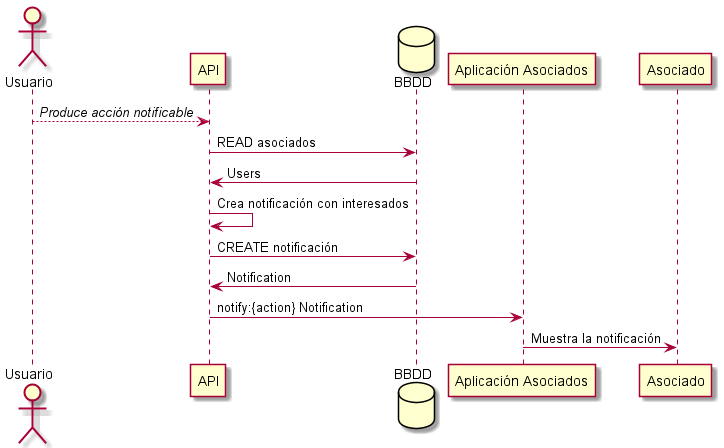
\includegraphics[width=0.75\textwidth]{images/Diseño/SecuenciaNotificaciones.png}
    \caption{Diagrama de secuencia del envío de notificaciones}
    \label{dia:secuencia_notificacion}
\end{figure}